\documentclass[conference,a4paper]{IEEEtran}
\IEEEoverridecommandlockouts
\usepackage{newtxtext}  % Times, as in the IEEE template
\usepackage[varvw]{newtxmath}
\usepackage{cite}
\usepackage{amsmath}
\usepackage{graphicx}
\usepackage{textcomp}
\usepackage{xcolor}
\usepackage{array}
\usepackage{multirow}
\usepackage{url}
\usepackage[hidelinks]{hyperref}
\graphicspath{{figures/}}
% Generated by scripts/make_figures.py from results/*.csv. Do not edit by hand.
\newcommand{\AddLastBaDij}{1.0}
\newcommand{\AddLastBaDijDK}{1.0}
\newcommand{\AddLastBaTwoFive}{2.2}
\newcommand{\AddLastBaTwoSix}{4.6}
\newcommand{\AddLastGridDij}{1.0}
\newcommand{\AddLastGridDijDK}{1.0}
\newcommand{\AddLastGridTwoFive}{4.3}
\newcommand{\AddLastGridTwoSix}{5.0}
\newcommand{\AddLastHubDij}{1.0}
\newcommand{\AddLastHubDijDK}{1.0}
\newcommand{\AddLastHubTwoFive}{3.3}
\newcommand{\AddLastHubTwoSix}{5.6}
\newcommand{\AddLastRandDij}{1.0}
\newcommand{\AddLastRandDijDK}{1.0}
\newcommand{\AddLastRandTwoFive}{3.1}
\newcommand{\AddLastRandTwoSix}{4.2}
\newcommand{\AddRatioMaxTwoFive}{4.4}
\newcommand{\AddRatioMaxTwoSix}{5.1}
\newcommand{\AddRatioMinTwoFive}{3.3}
\newcommand{\AddRatioMinTwoSix}{4.0}
\newcommand{\AllRatioMax}{8.7}
\newcommand{\AllRatioMin}{1.2}
\newcommand{\ChainNets}{CAL and NA}
\newcommand{\ChainPctA}{93.5}
\newcommand{\ChainPctB}{94.8}
\newcommand{\ChainRatioMax}{8.0}
\newcommand{\ChainRatioMin}{6.7}
\newcommand{\ChainRestMax}{53}
\newcommand{\ChainRestMin}{17}
\newcommand{\CmpLastBaDij}{14.2}
\newcommand{\CmpLastBaDijDK}{10.6}
\newcommand{\CmpLastBaTwoFive}{9.5}
\newcommand{\CmpLastBaTwoSix}{13.0}
\newcommand{\CmpLastGridDij}{9.0}
\newcommand{\CmpLastGridDijDK}{6.8}
\newcommand{\CmpLastGridTwoFive}{11.0}
\newcommand{\CmpLastGridTwoSix}{11.0}
\newcommand{\CmpLastHubDij}{16.2}
\newcommand{\CmpLastHubDijDK}{11.1}
\newcommand{\CmpLastHubTwoFive}{46.6}
\newcommand{\CmpLastHubTwoSix}{31.0}
\newcommand{\CmpLastRandDij}{17.1}
\newcommand{\CmpLastRandDijDK}{14.0}
\newcommand{\CmpLastRandTwoFive}{11.7}
\newcommand{\CmpLastRandTwoSix}{13.3}
\newcommand{\CmpRandTwentyDij}{15.5}
\newcommand{\CmpRandTwentyTwoFive}{9.7}
\newcommand{\CmpRandTwentyTwoSix}{14.9}
\newcommand{\CmpRangeBaTwoFiveMax}{12}
\newcommand{\CmpRangeBaTwoFiveMin}{10}
\newcommand{\CmpRangeBaTwoSixMax}{13}
\newcommand{\CmpRangeBaTwoSixMin}{11}
\newcommand{\CmpRangeRandTwoFiveMax}{12}
\newcommand{\CmpRangeRandTwoFiveMin}{10}
\newcommand{\CmpRangeRandTwoSixMax}{15}
\newcommand{\CmpRangeRandTwoSixMin}{12}
\newcommand{\CmpRatioMaxTwoFive}{2.66}
\newcommand{\CmpRatioMaxTwoSix}{2.15}
\newcommand{\CmpRatioMinTwoFive}{1.39}
\newcommand{\CmpRatioMinTwoSix}{1.63}
\newcommand{\CrossCmpBaTwoFiveDij}{16}
\newcommand{\CrossCmpBaTwoFiveDijDK}{20}
\newcommand{\CrossCmpBaTwoSixDij}{20}
\newcommand{\CrossCmpBaTwoSixDijDK}{none}
\newcommand{\CrossCmpGridTwoFiveDij}{none}
\newcommand{\CrossCmpGridTwoFiveDijDK}{none}
\newcommand{\CrossCmpGridTwoSixDij}{none}
\newcommand{\CrossCmpGridTwoSixDijDK}{none}
\newcommand{\CrossCmpHubTwoFiveDij}{none}
\newcommand{\CrossCmpHubTwoFiveDijDK}{none}
\newcommand{\CrossCmpHubTwoSixDij}{none}
\newcommand{\CrossCmpHubTwoSixDijDK}{none}
\newcommand{\CrossCmpRandTwoFiveDij}{14}
\newcommand{\CrossCmpRandTwoFiveDijDK}{17}
\newcommand{\CrossCmpRandTwoSixDij}{20}
\newcommand{\CrossCmpRandTwoSixDijDK}{22}
\newcommand{\CrossOpsBaTwoFiveDij}{18}
\newcommand{\CrossOpsBaTwoFiveDijDK}{none}
\newcommand{\CrossOpsBaTwoSixDij}{none}
\newcommand{\CrossOpsBaTwoSixDijDK}{none}
\newcommand{\CrossOpsGridTwoFiveDij}{none}
\newcommand{\CrossOpsGridTwoFiveDijDK}{none}
\newcommand{\CrossOpsGridTwoSixDij}{none}
\newcommand{\CrossOpsGridTwoSixDijDK}{none}
\newcommand{\CrossOpsHubTwoFiveDij}{none}
\newcommand{\CrossOpsHubTwoFiveDijDK}{none}
\newcommand{\CrossOpsHubTwoSixDij}{none}
\newcommand{\CrossOpsHubTwoSixDijDK}{none}
\newcommand{\CrossOpsRandTwoFiveDij}{16}
\newcommand{\CrossOpsRandTwoFiveDijDK}{18}
\newcommand{\CrossOpsRandTwoSixDij}{22}
\newcommand{\CrossOpsRandTwoSixDijDK}{none}
\newcommand{\DensHighTwoFive}{1.6}
\newcommand{\DensHighTwoSix}{2.3}
\newcommand{\DensLowTwoFive}{2.2}
\newcommand{\DensLowTwoSix}{3.6}
\newcommand{\DensMaxTwoFive}{2.2}
\newcommand{\DensMaxTwoSix}{3.6}
\newcommand{\DensMinTwoFive}{1.5}
\newcommand{\DensMinTwoSix}{2.3}
\newcommand{\DkLargeMax}{2.1}
\newcommand{\DupPctMaxTwoFive}{1.0}
\newcommand{\DupPctMaxTwoSix}{0.9}
\newcommand{\DupPctMinTwoFive}{0.1}
\newcommand{\DupPctMinTwoSix}{0.0}
\newcommand{\FaceValueCrossLog}{982}
\newcommand{\GainTwoFiveAtSixtyFour}{4.0}
\newcommand{\GainTwoFiveAtTwenty}{2.7}
\newcommand{\GainTwoSixAtSixtyFour}{3.3}
\newcommand{\GainTwoSixAtTwenty}{2.2}
\newcommand{\GridLateMax}{3.8}
\newcommand{\GridLateMin}{2.7}
\newcommand{\HubCmpDij}{14}
\newcommand{\HubCmpRatioMaxTwoFive}{2.9}
\newcommand{\HubCmpRatioMaxTwoSix}{2.2}
\newcommand{\HubCmpRatioMinTwoFive}{2.4}
\newcommand{\HubCmpRatioMinTwoSix}{1.9}
\newcommand{\HubCmpTwoFive}{38}
\newcommand{\HubCmpTwoSix}{26}
\newcommand{\HubRedCmpDij}{118}
\newcommand{\HubRedCmpTwoFive}{98}
\newcommand{\HubRedCmpTwoSix}{55}
\newcommand{\HubRedDijSlow}{6.7}
\newcommand{\HubRedSameTwoFive}{2.9}
\newcommand{\HubRedSameTwoSix}{2.5}
\newcommand{\MainScanMaxTwoFive}{2.8}
\newcommand{\MainScanMaxTwoSix}{4.0}
\newcommand{\MainScanMinTwoFive}{2.1}
\newcommand{\MainScanMinTwoSix}{3.0}
\newcommand{\MemDij}{501}
\newcommand{\MemRatioTwoFive}{1.7}
\newcommand{\MemRatioTwoSix}{2.3}
\newcommand{\MemTwoFive}{859}
\newcommand{\MemTwoSix}{1170}
\newcommand{\MsSixteenDij}{6}
\newcommand{\MsSixteenTwoFive}{11}
\newcommand{\MsTwentyDij}{271}
\newcommand{\MsTwentyTwoDij}{1866}
\newcommand{\MsTwentyTwoFive}{454}
\newcommand{\MsTwentyTwoTwoFive}{2805}
\newcommand{\OpsRandTwentyDij}{16.5}
\newcommand{\OpsRandTwentyTwoFive}{11.9}
\newcommand{\OpsRandTwentyTwoSix}{19.8}
\newcommand{\OpsRatioMaxTwoFive}{2.9}
\newcommand{\OpsRatioMaxTwoSix}{2.5}
\newcommand{\OpsRatioMinTwoFive}{1.6}
\newcommand{\OpsRatioMinTwoSix}{2.0}
\newcommand{\ParNATwoFiveBest}{3.94}
\newcommand{\ParNATwoFiveBestK}{6}
\newcommand{\ParNATwoFiveBestT}{5}
\newcommand{\ParNATwoFiveDefault}{6.44}
\newcommand{\ParNATwoFiveGain}{39}
\newcommand{\ParNATwoFiveWorst}{15.9}
\newcommand{\ParNATwoSixBest}{4.72}
\newcommand{\ParNATwoSixBestK}{4}
\newcommand{\ParNATwoSixBestT}{9}
\newcommand{\ParNATwoSixDefault}{6.80}
\newcommand{\ParNATwoSixGain}{31}
\newcommand{\ParNATwoSixWorst}{15.4}
\newcommand{\ParSFTwoFiveBest}{3.05}
\newcommand{\ParSFTwoFiveBestK}{5}
\newcommand{\ParSFTwoFiveBestT}{6}
\newcommand{\ParSFTwoFiveDefault}{3.46}
\newcommand{\ParSFTwoFiveGain}{12}
\newcommand{\ParSFTwoFiveWorst}{14.1}
\newcommand{\ParSFTwoSixBest}{4.09}
\newcommand{\ParSFTwoSixBestK}{3}
\newcommand{\ParSFTwoSixBestT}{9}
\newcommand{\ParSFTwoSixDefault}{4.62}
\newcommand{\ParSFTwoSixGain}{11}
\newcommand{\ParSFTwoSixWorst}{12.8}
\newcommand{\PeakBa}{51}
\newcommand{\PeakGrid}{0.1}
\newcommand{\PeakGridSmall}{7.5}
\newcommand{\PeakHub}{100}
\newcommand{\PeakRand}{33}
\newcommand{\PerOpMaxTwoFive}{2.9}
\newcommand{\PerOpMaxTwoSix}{2.7}
\newcommand{\PerOpMinTwoFive}{2.1}
\newcommand{\PerOpMinTwoSix}{2.3}
\newcommand{\PivotScanMaxTwoFive}{1.98}
\newcommand{\PivotScanMaxTwoSix}{0.72}
\newcommand{\PivotScanMinTwoFive}{1.16}
\newcommand{\PivotScanMinTwoSix}{0.02}
\newcommand{\PrintedTimeMaxTwoFive}{1.09}
\newcommand{\PrintedTimeMaxTwoSix}{1.01}
\newcommand{\PrintedTimeMinTwoFive}{0.98}
\newcommand{\PrintedTimeMinTwoSix}{0.97}
\newcommand{\RatioRandSixteenTwoFive}{1.9}
\newcommand{\RatioRandTwentyTwoFive}{1.7}
\newcommand{\RatioRandTwentyTwoTwoFive}{1.5}
\newcommand{\RealRatioMax}{8.0}
\newcommand{\RealRatioMaxTwoFive}{8.0}
\newcommand{\RealRatioMaxTwoSix}{6.7}
\newcommand{\RealRatioMin}{3.5}
\newcommand{\RealRatioMinTwoFive}{3.5}
\newcommand{\RealRatioMinTwoSix}{4.7}
\newcommand{\RealSources}{20}
\newcommand{\RealSrcMaxTwoFive}{9.5}
\newcommand{\RealSrcMaxTwoSix}{7.3}
\newcommand{\RealSrcMinTwoFive}{3.2}
\newcommand{\RealSrcMinTwoSix}{4.3}
\newcommand{\RealTwoSixFasterCount}{1}
\newcommand{\RealTwoSixFasterList}{CAL}
\newcommand{\RealTwoSixFasterWord}{one}
\newcommand{\RealTwoSixSlowerWord}{four}
\newcommand{\ReduceNGrowMax}{5.2}
\newcommand{\ReduceNGrowMin}{4.1}
\newcommand{\ReduceSlowMaxTwoFive}{5.6}
\newcommand{\ReduceSlowMaxTwoSix}{3.2}
\newcommand{\ReduceSlowMinTwoFive}{2.5}
\newcommand{\ReduceSlowMinTwoSix}{2.0}
\newcommand{\RestRatioMax}{5.1}
\newcommand{\RestRatioMin}{3.5}
\newcommand{\RoadPeakMax}{1.7}
\newcommand{\RoadPeakMin}{0.1}
\newcommand{\RoadsMoreAddsTwoSix}{four}
\newcommand{\RoadsMoreCmpTwoSix}{four}
\newcommand{\ScaleBaMaxExp}{21}
\newcommand{\ScaleBaTwoFiveArgmin}{21}
\newcommand{\ScaleBaTwoFiveFirst}{5.7}
\newcommand{\ScaleBaTwoFiveLast}{1.2}
\newcommand{\ScaleBaTwoFiveMax}{5.7}
\newcommand{\ScaleBaTwoFiveMin}{1.25}
\newcommand{\ScaleBaTwoSixArgmin}{21}
\newcommand{\ScaleBaTwoSixFirst}{6.3}
\newcommand{\ScaleBaTwoSixLast}{2.0}
\newcommand{\ScaleBaTwoSixMax}{6.3}
\newcommand{\ScaleBaTwoSixMin}{2.02}
\newcommand{\ScaleGridMaxExp}{22}
\newcommand{\ScaleGridTwoFiveArgmin}{18}
\newcommand{\ScaleGridTwoFiveFirst}{5.6}
\newcommand{\ScaleGridTwoFiveLast}{3.0}
\newcommand{\ScaleGridTwoFiveMax}{5.6}
\newcommand{\ScaleGridTwoFiveMin}{2.72}
\newcommand{\ScaleGridTwoSixArgmin}{18}
\newcommand{\ScaleGridTwoSixFirst}{6.0}
\newcommand{\ScaleGridTwoSixLast}{3.4}
\newcommand{\ScaleGridTwoSixMax}{6.0}
\newcommand{\ScaleGridTwoSixMin}{3.14}
\newcommand{\ScaleHubMaxExp}{21}
\newcommand{\ScaleHubTwoFiveArgmin}{21}
\newcommand{\ScaleHubTwoFiveFirst}{8.2}
\newcommand{\ScaleHubTwoFiveLast}{1.7}
\newcommand{\ScaleHubTwoFiveMax}{8.2}
\newcommand{\ScaleHubTwoFiveMin}{1.68}
\newcommand{\ScaleHubTwoSixArgmin}{21}
\newcommand{\ScaleHubTwoSixFirst}{8.7}
\newcommand{\ScaleHubTwoSixLast}{3.9}
\newcommand{\ScaleHubTwoSixMax}{8.7}
\newcommand{\ScaleHubTwoSixMin}{3.94}
\newcommand{\ScaleRandMaxExp}{22}
\newcommand{\ScaleRandTwoFiveArgmin}{22}
\newcommand{\ScaleRandTwoFiveFirst}{5.9}
\newcommand{\ScaleRandTwoFiveLast}{1.5}
\newcommand{\ScaleRandTwoFiveMax}{5.9}
\newcommand{\ScaleRandTwoFiveMin}{1.48}
\newcommand{\ScaleRandTwoSixArgmin}{22}
\newcommand{\ScaleRandTwoSixFirst}{6.8}
\newcommand{\ScaleRandTwoSixLast}{1.8}
\newcommand{\ScaleRandTwoSixMax}{6.8}
\newcommand{\ScaleRandTwoSixMin}{1.85}
\newcommand{\ScanLastBaDij}{1.0}
\newcommand{\ScanLastBaDijDK}{1.0}
\newcommand{\ScanLastBaTwoFive}{3.3}
\newcommand{\ScanLastBaTwoSix}{4.6}
\newcommand{\ScanLastGridDij}{1.0}
\newcommand{\ScanLastGridDijDK}{1.0}
\newcommand{\ScanLastGridTwoFive}{5.3}
\newcommand{\ScanLastGridTwoSix}{5.0}
\newcommand{\ScanLastHubDij}{1.0}
\newcommand{\ScanLastHubDijDK}{1.0}
\newcommand{\ScanLastHubTwoFive}{4.0}
\newcommand{\ScanLastHubTwoSix}{5.6}
\newcommand{\ScanLastRandDij}{1.0}
\newcommand{\ScanLastRandDijDK}{1.0}
\newcommand{\ScanLastRandTwoFive}{4.1}
\newcommand{\ScanLastRandTwoSix}{4.2}
\newcommand{\ScanMaxTwoFive}{4.8}
\newcommand{\ScanMaxTwoSix}{5.1}
\newcommand{\ScanMinTwoFive}{4.3}
\newcommand{\ScanMinTwoSix}{4.0}
\newcommand{\SlopeBaDij}{0.67}
\newcommand{\SlopeBaDijDK}{0.50}
\newcommand{\SlopeBaTwoFive}{-0.22}
\newcommand{\SlopeBaTwoSix}{0.09}
\newcommand{\SlopeGridDij}{0.33}
\newcommand{\SlopeGridDijDK}{0.26}
\newcommand{\SlopeGridTwoFive}{0.30}
\newcommand{\SlopeGridTwoSix}{0.16}
\newcommand{\SlopeHubDij}{0.75}
\newcommand{\SlopeHubDijDK}{0.50}
\newcommand{\SlopeHubTwoFive}{2.65}
\newcommand{\SlopeHubTwoSix}{0.96}
\newcommand{\SlopeRandDij}{0.80}
\newcommand{\SlopeRandDijDK}{0.67}
\newcommand{\SlopeRandTwoFive}{0.14}
\newcommand{\SlopeRandTwoSix}{-0.07}
\newcommand{\SnapBestInstance}{Pokec with random weights}
\newcommand{\SnapCmpOtherMaxTwoFive}{1.65}
\newcommand{\SnapCmpOtherMaxTwoSix}{2.91}
\newcommand{\SnapCmpOtherMinTwoFive}{0.79}
\newcommand{\SnapCmpOtherMinTwoSix}{1.23}
\newcommand{\SnapCmpRoadMaxTwoFive}{1.43}
\newcommand{\SnapCmpRoadMaxTwoSix}{1.61}
\newcommand{\SnapCmpRoadMinTwoFive}{1.09}
\newcommand{\SnapCmpRoadMinTwoSix}{1.22}
\newcommand{\SnapFewerCmpDKTwoFive}{none}
\newcommand{\SnapFewerCmpDKTwoSix}{none}
\newcommand{\SnapFewerCmpTwoFive}{two}
\newcommand{\SnapFewerCmpTwoSix}{none}
\newcommand{\SnapFewerListTwoFive}{Google and Pokec}
\newcommand{\SnapGraphs}{six}
\newcommand{\SnapInstances}{twelve}
\newcommand{\SnapOtherPeakMax}{50}
\newcommand{\SnapOtherPeakMin}{13}
\newcommand{\SnapRandCmpMaxTwoFive}{1.20}
\newcommand{\SnapRandCmpMaxTwoSix}{1.52}
\newcommand{\SnapRandCmpMinTwoFive}{0.79}
\newcommand{\SnapRandCmpMinTwoSix}{1.22}
\newcommand{\SnapRandTimeMaxTwoFive}{3.1}
\newcommand{\SnapRandTimeMaxTwoSix}{4.3}
\newcommand{\SnapRandTimeMinTwoFive}{1.3}
\newcommand{\SnapRandTimeMinTwoSix}{1.9}
\newcommand{\SnapRatioMaxTwoFive}{3.2}
\newcommand{\SnapRatioMaxTwoSix}{4.5}
\newcommand{\SnapRatioMinTwoFive}{1.3}
\newcommand{\SnapRatioMinTwoSix}{1.9}
\newcommand{\SnapRoadPeakMax}{0.3}
\newcommand{\SnapTimeOtherMaxTwoFive}{3.2}
\newcommand{\SnapTimeOtherMaxTwoSix}{4.5}
\newcommand{\SnapTimeOtherMinTwoFive}{1.3}
\newcommand{\SnapTimeOtherMinTwoSix}{1.9}
\newcommand{\SnapTimeRoadMaxTwoFive}{3.0}
\newcommand{\SnapTimeRoadMaxTwoSix}{3.8}
\newcommand{\SnapTimeRoadMinTwoFive}{2.6}
\newcommand{\SnapTimeRoadMinTwoSix}{3.3}
\newcommand{\SnapTwoSixFaster}{none}
\newcommand{\SnapUnitCmpMaxTwoFive}{1.65}
\newcommand{\SnapUnitCmpMaxTwoSix}{2.91}
\newcommand{\SnapUnitCmpMinTwoFive}{1.03}
\newcommand{\SnapUnitCmpMinTwoSix}{1.56}
\newcommand{\SnapUnitTimeMaxTwoFive}{3.2}
\newcommand{\SnapUnitTimeMaxTwoSix}{4.5}
\newcommand{\SnapUnitTimeMinTwoFive}{2.2}
\newcommand{\SnapUnitTimeMinTwoSix}{3.0}
\newcommand{\SynthPoints}{44}
\newcommand{\SynthTwoSixFasterCount}{0}
\newcommand{\TimeRandTwentyTwoFive}{1.7}
\newcommand{\TimeRandTwentyTwoSix}{2.7}
\newcommand{\ValMediumBoundTwoSix}{1\,435}
\newcommand{\ValMediumDupTwoFive}{9\,343}
\newcommand{\ValMediumDupTwoSix}{10\,510}
\newcommand{\ValMediumRuns}{510\,000}
\newcommand{\ValMediumStaleTwoFive}{10\,402}
\newcommand{\ValMediumStaleTwoSix}{10\,510}
\newcommand{\ValMediumTrials}{30\,000}
\newcommand{\ValMediumWrong}{0}
\newcommand{\ValMinNBoundTwoSix}{10}
\newcommand{\ValMinNDupTwoFive}{9}
\newcommand{\ValMinNDupTwoSix}{12}
\newcommand{\ValSmallBoundTwoSix}{8\,939}
\newcommand{\ValSmallDupTwoFive}{4\,788}
\newcommand{\ValSmallDupTwoSix}{3\,475}
\newcommand{\ValSmallRuns}{3\,400\,000}
\newcommand{\ValSmallStaleTwoFive}{5\,293}
\newcommand{\ValSmallStaleTwoSix}{3\,475}
\newcommand{\ValSmallTrials}{200\,000}
\newcommand{\ValSmallWrong}{0}
\newcommand{\WeightMaxTwoFive}{2.3}
\newcommand{\WeightMaxTwoSix}{3.8}
\newcommand{\WeightMinTwoFive}{1.9}
\newcommand{\WeightMinTwoSix}{2.8}
\newcommand{\WeightUnitTwoFive}{1.9}
\newcommand{\WeightUnitTwoSix}{2.8}
\newcommand{\WeightWideTwoFive}{1.9}
\newcommand{\WeightWideTwoSix}{3.0}

% \input is not expandable enough inside a tabular; use the primitive for table bodies.
\makeatletter\newcommand{\tabinput}[1]{\@@input #1 }\makeatother

% Author block: all authors share one affiliation, so a single block is used (names, department,
% university, location, e-mail addresses in the order of the names).
\newcommand{\dhat}{\widehat{d}}
\newcommand{\Bp}{B'}
\newcommand{\bmA}{BMSSP-25}
\newcommand{\bmB}{BMSSP-26}
\newcommand{\fp}{\textsc{FindPivots}}
\newcommand{\Oh}{O}

\renewcommand{\IEEEkeywordsname}{Keywords}
% "Abstract." and "Keywords." with a full stop instead of the em dash that IEEEtran puts after them.
\usepackage{etoolbox}
\makeatletter
\patchcmd{\abstract}{---}{.\ }{}{\PackageWarning{main}{abstract heading not patched}}
\patchcmd{\IEEEkeywords}{---}{.\ }{}{\PackageWarning{main}{keywords heading not patched}}
\makeatother
\begin{document}

\title{A Comprehensive Theoretical and Experimental Comparison of Dijkstra's Algorithm and
Duan~et~al.'s SSSP Algorithms}

\author{\IEEEauthorblockN{Anmol, Tanmay Arora, Adhyyan, Pahul Veer Singh Gogna}
\IEEEauthorblockA{\textit{Department of Computer Science \& Engineering}\\
\textit{Chitkara University}\\
Punjab, India\\
anmol0115.be23@chitkara.edu.in, tanmay1305.be23@chitkara.edu.in,\\
adhyyan0180.be23@chitkara.edu.in, pahul0508.be23@chitkara.edu.in}}

\maketitle

\begin{abstract}
Dijkstra's algorithm has been widely used as the standard practical method for the single source
shortest path (SSSP) problem for nearly six decades, but its dominant position has recently been
challenged. In 2025 the first deterministic algorithm for directed graphs with nonnegative real
weights that is asymptotically faster on sparse graphs was introduced by Duan, Mao, Mao, Shu and
Yin, and in 2026 this approach was further refined by Duan, Mao, Shu and Yin, who presented an
improved algorithm with a better theoretical bound. Although both algorithms are primarily
theoretical, their potential impact is significant. In this study all three algorithms were
comprehensively compared under identical conditions: a component-by-component comparison of the
two new algorithms was conducted, both were implemented directly from their published pseudocode,
and they were validated on \ValSmallTrials{} and \ValMediumTrials{} random graphs. Running time
and machine-independent counts of comparisons, additions and edge scans were carefully evaluated
on eleven real world graphs and four synthetic families, some containing up to four million
vertices. Dijkstra's algorithm, particularly when implemented with a binary heap, consistently
achieved the best performance across all instances; on the five major road networks it was
\RealRatioMin{} to \RealRatioMax{} times faster than the other algorithms. On random and
preferential-attachment graphs, where a wide search frontier is typically encountered, the
earlier of the two new algorithms required fewer comparisons than Dijkstra's algorithm on large
graphs, demonstrating its asymptotic advantage under the theoretical cost model; nevertheless, at
four million vertices it was still approximately \ScaleRandTwoFiveLast{} times slower than
Dijkstra's algorithm. The later algorithm attempts to reduce much of the pivot-search overhead of
the earlier version, but surprisingly it was faster than its predecessor on only
\RealTwoSixFasterWord{} instance. Instrumented runs also detected a previously known stale-key
error of the earlier algorithm, which, alarmingly, also appears in the published pseudocode of
the later one, and its base case can return a boundary that violates its own invariant;
fortunately, neither issue affected any computed distance.
\end{abstract}

\begin{IEEEkeywords}
single source shortest paths, Dijkstra's algorithm, bounded multi-source shortest path, sorting
barrier, experimental algorithmics, comparison-addition model
\end{IEEEkeywords}

\section{Introduction}
The single source shortest path (SSSP) problem is a fundamental problem in graph theory: the
shortest path distances from a designated source vertex $s$ to all other vertices of a directed
graph $G=(V,E)$ are required, where the graph has $n=|V|$ vertices and $m=|E|$ directed arcs with
nonnegative real weights on every arc. A solution was first provided by Dijkstra's
algorithm~\cite{dijkstra1959}: when a Fibonacci heap~\cite{fredman1987} or a relaxed
heap~\cite{driscoll1988} is used to manage the frontier, a running time of $\Oh(m+n\log n)$ is
achieved, in the comparison-addition model in which weights can only be added and compared. A key
characteristic of Dijkstra's algorithm is that the vertices are settled in order of increasing
distance from the source, so they are effectively sorted as a side product, and for a long time
the $n\log n$ term was regarded as an unavoidable barrier for sparse graphs. This intuition was
later clarified by Haeupler et al.~\cite{haeupler2024}: an appropriate heap implementation of
Dijkstra's algorithm was shown to be universally optimal among the algorithms that must produce
the vertices in distance order. This distinction is important, because an algorithm that returns
only the distances, without producing the vertices in sorted order, is not subject to the same
limitation.

This limitation was addressed by Duan, Mao, Mao, Shu and Yin~\cite{duan2025}. A deterministic
algorithm with a running time of $\Oh(m\log^{2/3}n)$ was introduced, the first to surpass the
$\Oh(m+n\log n)$ barrier on sparse directed graphs with real weights. Its central innovation is a
recursive technique, the bounded multi-source shortest path (BMSSP) procedure, in which the whole
frontier is not kept sorted: instead, the frontier is reduced to a small collection of pivots
through a specialized subroutine, and a block-based structure distributes the smallest frontier
elements without ordering them internally. In 2026 this approach was significantly developed by
Duan, Mao, Shu and Yin~\cite{duan2026}: an improved bound of $\Oh(m\sqrt{\log n}+\sqrt{mn\log n
\log\log n})$, which simplifies to $\Oh(m\sqrt{\log n\log\log n})$ for sparse graphs, was
established by replacing the Bellman Ford style pivot search with local Dijkstra searches and a
forest partition and by simplifying the data structure. Since neither paper assigns a name to its
algorithm, the algorithm of Duan, Mao, Mao, Shu and Yin~\cite{duan2025} is referred to here as
\bmA{} and the improved algorithm of Duan, Mao, Shu and Yin~\cite{duan2026} as \bmB{}, where the
suffix indicates the year of publication.

Neither paper provides a detailed discussion of practical implementation. Nevertheless, an
experimental evaluation is valuable for three main reasons. First, the asymptotic improvement is
relatively modest: $\log^{1/3}n$ is \GainTwoFiveAtTwenty{} for $n=2^{20}$ and increases to only
\GainTwoFiveAtSixtyFour{} for $n=2^{64}$, so a theoretical advantage need not translate into
better practical performance unless the constant factors are carefully controlled. Second,
potentially large constant factors are involved in both algorithms, since the arcs must be
scanned several times and highly specialized, custom-built data structures must be maintained.
Third, the assumptions underlying the analyses are not straightforward to satisfy in practice:
both rely on a degree-bounded graph obtained through a transformation, and both require distinct
path lengths, which are generally ensured through tie-breaking. \bmA{} has already been evaluated
in earlier studies~\cite{castro2025,valko2025,makowski2025}; to the best of our knowledge,
however, no peer reviewed empirical evaluation of \bmB{} has yet been published, and the
algorithms have not previously been evaluated in the same model in which their running time
bounds were originally established.

The following contributions are presented in this paper.
\begin{itemize}
\item A detailed, component-by-component comparison of Dijkstra's algorithm, \bmA{} and \bmB{} is
provided, with particular attention to the parameter values the algorithms use at practical input
sizes (Section~\ref{sec:theory}).
\item Independent C++ implementations of both BMSSP algorithms were developed directly from the
published pseudocode, and randomized differential testing was conducted to validate their
correctness (Sections~\ref{sec:impl} and~\ref{sec:correct}).
\item Two issues in the published pseudocode of \bmB{} were identified during validation:
completed vertices can remain stored in the caller's data structure, as in \bmA, and the base
case can return a boundary greater than a value it leaves behind (Section~\ref{sec:correct}).
\item Extensive measurements of running time, comparisons, additions and edge scans were
conducted on five real road networks, six further graphs from the SNAP collection and four
synthetic families, with sweeps over the parameters $k$ and $t$ and over the degree reduction,
density and weight range (Section~\ref{sec:results}).
\end{itemize}

\section{Related Work}
\subsection{Classical results}
An $\Oh(m+n\log n)$ running time bound for Dijkstra's algorithm was established by Fredman and
Tarjan~\cite{fredman1987} through Fibonacci heaps, and this result was complemented by the
relaxed heaps of Driscoll et al.~\cite{driscoll1988}. Experimental research on shortest path
algorithms has a long tradition~\cite{cherkassky1996}, and in practice Dijkstra's algorithm is
generally equipped with a binary heap, as in~\cite{castro2025}. Faster algorithms have been
developed, although they generally fall outside the scope of the present study: Thorup's
linear-time algorithm~\cite{thorup1999} is restricted to undirected graphs with integer weights
in the word RAM model, and the algorithm of Pettie and Ramachandran~\cite{pettie2005} is also
designed for undirected graphs. For undirected graphs with real weights, a randomized
$\Oh(m\sqrt{\log n\log\log n})$ algorithm was introduced by Duan et al.~\cite{duan2023} and later
derandomized by Yan~\cite{yan2026}; a further improvement for undirected graphs appeared while
the present study was being prepared~\cite{kadria2026}.

\subsection{Experimental studies of \bmA}
\bmA{} was implemented in C++ by Castro, Clementino and de Freitas~\cite{castro2025} in three
variants (worst case, constant degree, expected time). The first variant was compared with
binary-heap Dijkstra on sparse random graphs containing up to $2^{25}$ vertices, as well as on
grids and United States road networks. Dijkstra's algorithm was observed to be three to four
times faster on large instances and up to 27.5 times faster on small grids. Through curve
fitting, a potential crossover point was estimated to lie far beyond any practical size, and the
constant-degree transformation was concluded to be detrimental to practical performance. A
critical error in the original analysis was also identified: a vertex already completed within a
recursive call could remain in the data structure with an outdated key, so the sets returned by
successive calls were not necessarily disjoint; this was resolved by removing each vertex
immediately upon completion, and both the problem and the correction were confirmed by the
original authors~\cite{castro2025}. Their implementation was made publicly available~\cite{bmsspcode}.
A Rust implementation was evaluated by Valko, Paranjpe and Marx G\'omez~\cite{valko2025} on
snapshots of the Lightning Network, and Dijkstra's algorithm was likewise found to be faster. A
Python package was provided by Makowski et al.~\cite{makowski2025}, through which measurements on
grid and geospatial networks were also reported.

Several public repositories have also claimed to implement \bmA, with some reporting better
performance than Dijkstra's algorithm~\cite{ryu2025,webb2025}. Closer examination of their source
code, however, reveals that these results often concern variants that differ from the published
algorithm. For example, the optimized solver of~\cite{ryu2025} replaces the recursion over
levels, the pivot search and the block structure with a bucket queue of fixed bucket width, and
it was evaluated on queries from one source to one target in unit-weight graphs, where distance-based
bucketing achieves linear-time performance outside the comparison-addition model; the same
repository reports that its solver which follows the paper more closely is two to four times
slower than Dijkstra. Similarly, the comparison in~\cite{webb2025} concerns queries from one
source to one target on unit-weight graphs against a standard library routine. These results are therefore not
considered direct measurements of the algorithm of~\cite{duan2025}, but the graphs used in these
studies were included in our experiments (Section~\ref{sec:setup}).

The studies above primarily report the wall clock running time of \bmA{} (with memory also
reported in~\cite{castro2025}). Several important questions remain open, however: how \bmB{}
performs in practice, how much of the observed gap is attributable to additional algorithmic work
rather than the cost of individual operations, and how performance depends on graph structures
beyond random graphs, grids and road networks.

\section{The Three Algorithms}\label{sec:theory}
\subsection{A common view}
All three algorithms maintain tentative labels $\dhat[v]\ge d(v)$, where $d(v)$ is the true
shortest path distance to $v$, and a label is reduced only when an arc $(u,v)$ is relaxed, that
is, by setting $\dhat[v]\leftarrow\dhat[u]+w_{uv}$. A vertex is \emph{complete} when
$\dhat[v]=d(v)$. Following~\cite{duan2026}, each algorithm maintains a \emph{frontier}: a set of
vertices such that the shortest path to every incomplete vertex passes through a complete
frontier vertex. Repeatedly, a set $Z$ of complete vertices is identified, the arcs leaving $Z$
are relaxed, and the vertices of $Z$ are replaced in the frontier by the out-neighbours just
improved. The algorithms differ in how the set $Z$ is identified and selected.

In Dijkstra's algorithm, $Z$ is the single frontier vertex with the smallest label, which is
necessarily complete. A priority queue over the whole frontier is therefore required, and when
the frontier contains $\Theta(n)$ vertices each extraction incurs $\Theta(\log n)$ comparisons.

Both BMSSP algorithms instead solve the subproblem $\textsc{BMSSP}(l,B,S)$: given a level $l$, a
bound $B$ and a frontier $S$, all vertices $v$ with $d(v)<B$ whose shortest path visits $S$ are to
be completed. During a call, the part $S_i$ of the frontier lying below a separator $B_i$ is
extracted, the subproblem $(l-1,B_i,S_i)$ is solved recursively, the arcs out of the returned
complete set $U_i$ are relaxed, and the process is repeated. A call may stop early (a
\emph{partial} execution) once enough vertices have been completed, returning a boundary $\Bp<B$
up to which its work is final. The whole problem is the initial call with $S=\{s\}$, $B=\infty$ at
level $\lceil(\log n)/t\rceil$. Table~\ref{tab:theory} lists the components.

\begin{table*}[t]
\caption{Components of the three algorithms}
\label{tab:theory}
\centering
\renewcommand{\arraystretch}{1.15}
\begin{tabular}{@{}p{2.4cm}p{3.2cm}p{5.4cm}p{5.6cm}@{}}
\hline
 & Dijkstra~\cite{dijkstra1959,fredman1987} & \bmA~\cite{duan2025} & \bmB~\cite{duan2026}\\
\hline
Running time
  & $\Oh(m+n\log n)$
  & $\Oh(m\log^{2/3}n)$
  & $\Oh(m\sqrt{\log n}+\sqrt{mn\log n\log\log n})$\\
Output
  & distances in sorted order
  & distances
  & distances\\
Complete set $Z$
  & minimum of the frontier
  & set $U_i$ returned by a recursive call
  & set $U_i$ returned by a recursive call\\
Frontier reduction
  & none
  & pivots: roots of shortest path trees with at least $k$ vertices; at most $|U|/k$ of
    them
  & one representative (the minimum) per subtree of $\Theta(k)$ vertices of a forest
    spanning $S$\\
Pivot finding
  & -
  & $k$ rounds of Bellman Ford relaxation from $S$: $\Oh(k)$ per vertex
  & local Dijkstra searches that stop after $k$ vertices, then a linear-time partition:
    $\Oh(\log k)$ per vertex\\
Partial sorting
  & heap (total order)
  & two block sequences; \textsc{Insert} in $\Oh(\log(N/M))$, \textsc{BatchPrepend},
    \textsc{Pull}
  & one search tree of blocks; \textsc{Insert} in $\Oh(\log(N/M))$, linear-time
    \textsc{Merge} and \textsc{Pull}\\
Hand-back after a partial call
  & -
  & caller reinserts what it can reconstruct (\textsc{BatchPrepend})
  & callee returns its remaining frontier $D$; caller merges it\\
Call stops when
  & frontier empty
  & $|U|\ge k2^{lt}$ or $D$ empty
  & $|U|>t^32^{lt}$ or $D$ empty\\
Base case ($l=0$)
  & -
  & Dijkstra from one vertex, $k+1$ vertices
  & Dijkstra from a set, $t^3+1$ vertices\\
Parameters
  & -
  & $k=\lfloor\log^{1/3}n\rfloor$, $t=\lfloor\log^{2/3}n\rfloor$
  & $t=\lceil\sqrt{\log n\log\log n/\delta}\,\rceil$, $k=\lceil t/\log t\rceil$\\
Degree assumption
  & none
  & in- and out-degree at most 2
  & degree at most $\delta$, $3\le\delta\le m/n$\\
\hline
\end{tabular}
\end{table*}

\subsection{\bmA: the algorithm of Duan, Mao, Mao, Shu and Yin}
\fp{} of \bmA{} relaxes outward from $S$ for $k$ rounds, restricted to the labels below $B$, and
collects every vertex it encounters in $W$. A key decision is then made from the sizes of $W$ and
$S$: if $|W|>k|S|$, the frontier is considered small relative to the remaining work, and every
vertex of $S$ is selected as a pivot. Otherwise, the tight arcs inside $W$ form a forest, and
only the roots in $S$ of trees having at least $k$ vertices are selected as pivots: a vertex whose
shortest path leaves $S$ through a smaller tree would already have been completed during the $k$
rounds. The selected pivots are inserted into a specialized structure $D$ that returns, for each
\textsc{Pull}, at most $M=2^{(l-1)t}$ keys of smallest value together with a separator. The
vertices improved by relaxing out of $U_i$ are then processed according to their new values: a
vertex is inserted individually if its new value is at least $B_i$, and prepended as part of a
batch if the value lies in $[\Bp_i,B_i)$. According to the analysis~\cite{duan2025}, \fp{} incurs
a cost of $\Oh(k)$ per vertex and level and the structure $\Oh(t)$ per insertion, and the two are
balanced by choosing $k=\lfloor\log^{1/3}n\rfloor$ and $t=\lfloor\log^{2/3}n\rfloor$.

\subsection{\bmB: the algorithm of Duan, Mao, Shu and Yin}
The central observation underlying \bmB{} is that the $k$ relaxation rounds make it possible to
determine, for each vertex, the pivot tree to which it belongs, which is more information than the
recursion strictly requires~\cite{duan2026}. \fp{} now runs a Dijkstra search from each $x\in S$,
terminating either once $k$ vertices have been discovered or once a tree built by an earlier
search is encountered, in which case the two trees are merged. If all reachable vertices are
processed before $k$ of them are found, $x$ is added to a set $Q$ and its vertices to $W$; these
are excluded from the recursion and processed collectively at the end of the call. The remaining
trees are partitioned by their edges into subtrees of between $k$ and $3k$
vertices~\cite{frederickson1983}, the frontier vertices of each subtree form a group $P_j$, and
only the vertex $p_j$ of smallest key in each group is inserted into $D$. When $p_j$ is pulled,
the members of $P_j$ below the separator are identified through a scan of the group and added to
$S_i$. The structure is organized around a single search tree of blocks, each containing
$M=t\,2^{(l-1)t}$ keys, and the remaining frontier of a call is returned in this form, allowing
the caller to merge it in linear time. For a graph of maximum degree $\delta$, a running time of
$\Oh(m(t+\log n\log t/(\delta t)))$ is obtained, which is minimized by
$t=\lceil\sqrt{\log n\log\log n/\delta}\,\rceil$.

\subsection{Preconditions}
\emph{Distinct path lengths.} Both analyses rely on the assumption that no two paths have the
same length. To ensure this, both papers compare the labels lexicographically as tuples
$\langle$length, number of arcs, vertex, predecessor$\rangle$. Each label therefore consists of
four distinct fields, and more than one field may need to be examined during a comparison, in
sharp contrast with Dijkstra's algorithm, in which comparisons are made on single numerical
values.

\emph{Bounded degree.} The analysis of \bmA{} is based on a graph in which every vertex has at
most two incoming and two outgoing arcs, obtained by replacing each original vertex with a cycle
of zero-weight arcs having one cycle vertex for each incident arc~\cite{duan2025,frederickson1983}.
The resulting graph contains at most $2m$ vertices and $3m$ arcs. \bmB{} generalizes the
construction to cycles of
$\lceil\Delta_v/(\delta-2)\rceil$ vertices for a vertex having $\Delta_v$ incident arcs and
requires $3\le\delta\le m/n$. The value which is proposed for $\delta$ is $\min\{m/n,\log\log
n\}/4$~\cite{duan2026}, which reaches the required minimum of three only when $\log\log n\ge 12$,
that is, for $n\ge 2^{4096}$; the authors note that the constants can be adjusted by the
implementers. For every feasible input the prescription therefore comes down to $\delta=3$ (or
to no reduction at all when $m/n<3$), and we use $\delta=3$ in the formula for $t$ everywhere.

\subsection{Parameters at feasible sizes}
Table~\ref{tab:params} evaluates the prescribed parameters. For all of the sizes which fit in
memory today \bmA{} uses $k\in\{2,3\}$, so its \fp{} performs two or three relaxation rounds,
and three or four recursion levels; \bmB{} also uses $k\in\{2,3\}$, so each local search stops
after two or three vertices, and its base case is a Dijkstra search over a few hundred vertices.
The last two columns give the factor by which each of the bounds improves on $n\log n$ for
sparse graphs when all of the hidden constants are set to one. Read this way the bound of \bmA{}
is the smaller of the two until $(\log\log n)^3<\log n$, that is, until $\log n$ exceeds
\FaceValueCrossLog{}. At any feasible size it is the constants that decide the comparison, and
this is what the experiments measure.

\begin{table}[t]
\caption{Prescribed parameters for concrete $n$ ($\delta=3$). Levels $=\lceil\log_2 n/t\rceil$;
gain $=$ factor by which the bound of the algorithm improves on $n\log n$ with unit constants}
\label{tab:params}
\centering
\setlength{\tabcolsep}{3.5pt}
\begin{tabular}{@{}c|cccc|ccccc@{}}
\hline
 & \multicolumn{4}{c|}{\bmA} & \multicolumn{5}{c}{\bmB}\\
$n$ & $k$ & $t$ & levels & gain & $k$ & $t$ & levels & $t^3$ & gain\\
\hline
\tabinput{tables/theory_params.tex}
\hline
\end{tabular}
\end{table}

\section{Implementation}\label{sec:impl}
All of the algorithms are implemented in C++17 in a single code base and share the graph
representation
(compressed sparse rows), the label type and the timing harness. The \bmA{} and \bmB{}
implementations were written from the pseudocode of~\cite{duan2025} and~\cite{duan2026}; no code
from other implementations was used.

\emph{Dijkstra.} Two variants are considered: a binary heap~\cite{williams1964} of (key, vertex)
pairs with lazy deletion referred to as Dijkstra, and an
indexed binary heap supporting \textsc{DecreaseKey}, referred to as Dijkstra-DK. Both algorithms use standard
path lengths. The former serves as the baseline for all comparisons and was found to be slightly faster than
\texttt{std::priority\_queue} on the two tested instances
(SF and a random graph with $2^{20}$ vertices).

\emph{Labels.} The BMSSP implementations store a 16-byte label (length, number of arcs,
predecessor) for each vertex and compare the tuples which are described in
Section~\ref{sec:theory}. Arc weights are 64-bit integers, so the sums are exact and the results
of the different algorithms can be compared for equality.

\emph{Partial-sorting structures.} Blocks are arrays having constant-time deletion by swapping
with the last element. The block index is a red-black tree~\cite{guibas1978} (\texttt{std::map}) keyed by the upper
bounds of the blocks, as proposed in both of the papers. A direct-address table
for each recursion level maps a vertex to its block and position, as in~\cite{castro2025}; this
is possible because the calls on one level run one after the other. Selection of the element of
a given rank, which is needed by \textsc{Pull}, block splits and \textsc{BatchPrepend}, uses
quickselect which switches to median-of-medians pivots~\cite{blum1973} once a linear work budget
is exceeded~\cite{musser1997}, so that the worst case stays linear. The base case of \bmB{} uses
a balanced search tree (\texttt{std::set}), as is prescribed by its pseudocode, and the local
searches of both algorithms use binary heaps in place of Fibonacci heaps; with at most $k+1$,
respectively $k+\delta$, entries this does not change any bound which matters at the sizes that
we consider.

\emph{Sets.} The sets $U$ which are returned by recursive calls are stored as contiguous ranges
of one global array, so returning a set costs nothing and the set of a caller is the
concatenation of the ranges of its children. Membership tests use time-stamped arrays.

\emph{Deviations from the pseudocode.} Three places are implemented in a different way from the
printed pseudocode. They can be switched on and off, and Section~\ref{sec:correct} reports what
each one of them changes. (i) In both algorithms a vertex is deleted from the $D$ of the caller
when a recursive call reports it as complete. For \bmA{} this is the repair of~\cite{castro2025}.
(ii) The base case of \bmB{} returns the smallest value which remains in its structure after the
loop in place of the separator of its last \textsc{Pull}. (iii) Line~28 of the main procedure of
\bmB{} selects a new representative only for the groups $P_j$ which are still nonempty, as the
accompanying text of~\cite{duan2026} says; a group can be emptied by later vertices of the same
$U_i$ after it was scheduled for reselection.

\emph{Counters.} A second build of the same sources increments counters for label or key
comparisons, additions $\dhat[u]+w_{uv}$, edge scans (split by the place where they occur), and
structure operations. Comparisons include the ones made inside heaps, search trees and
selection. The timing build has no instrumentation in it.

The implementations, the experiment drivers, the raw measurements and the scripts which
regenerate every table and figure of this paper from them are publicly
available~\cite{thiscode}.

\section{Experimental Setup}\label{sec:setup}
\emph{Road networks.} The real inputs are the five road networks of the SSTD~2005
collection~\cite{li2005}, which were obtained from the public mirror~\cite{ansari2020}:
Oldenburg (OL), San Joaquin County (TG), California (CAL), San Francisco (SF) and North America
(NA); OL, TG and SF come from the generator data of Brinkhoff~\cite{brinkhoff2002}. Each file
lists a road segment once along with its Euclidean length. All of the five networks are
connected when the segments are read as undirected, but a search which follows the segments only
in their listed direction reaches as few as six vertices from vertex~0 of CAL, so every segment
is entered as two opposite arcs. The lengths are given with six decimals and are multiplied by
$10^6$ to get exact integers. Table~\ref{tab:data} lists the resulting graphs.

\begin{table}[t]
\caption{Road networks (arcs counted in both directions). Front.: largest number of vertices
held at once by Dijkstra's heap, in percent of $n$. Last columns: prescribed $k/t/$levels}
\label{tab:data}
\centering
\setlength{\tabcolsep}{3pt}
\begin{tabular}{@{}lrrrrrcc@{}}
\hline
 & $n$ & $m$ & max & $m/n$ & front. & \bmA & \bmB\\
 &  &  & deg. &  & (\%) & \multicolumn{2}{c}{$k/t/$levels}\\
\hline
\tabinput{tables/datasets.tex}
\hline
\end{tabular}
\end{table}

\emph{SNAP graphs.} To cover larger real graphs of other kinds we add \SnapGraphs{} graphs of the
SNAP collection~\cite{snap}, all of which are also used in~\cite{ryu2025}: the web graphs
web-Stanford and web-Google, the road networks of Pennsylvania, Texas and California, and the
Pokec social network (Table~\ref{tab:snap}). The road files list both of the directions of every
road; all of the files are used as they are given. They have no weights, so every graph is run
twice, once with unit weights as in~\cite{ryu2025} and once with uniform random integer weights
in $[1,2^{20}]$. Since a random vertex of a directed web graph may reach almost nothing, the
sources are random vertices which reach at least a quarter of the graph.

\emph{Synthetic families.} Four families having $n$ from $2^{10}$ to $2^{22}$ extend the range of
sizes and structures: (i) random digraphs having a random Hamiltonian cycle and $2n$ further
uniformly random arcs ($m=3n$); (ii) square grids having arcs in both directions; (iii)
preferential-attachment graphs~\cite{barabasi1999} with two links for each new vertex, entered in
both directions, which have a heavy-tailed degree distribution; and (iv) hub graphs, which are
random digraphs in which the source also has an arc to every other vertex whose weight is larger
than every ordinary weight, so that the search starts with all of the $n$ vertices in its
frontier. Weights are uniform integers in $[1,2^{20}]$ unless they are varied. Two sweeps on
random digraphs having $n=2^{18}$ vary the average out-degree from 2 to 32 and the largest weight
from $1$ (all of the paths of equal hop count tie) to $2^{30}$.

\emph{Measures.} We report the wall clock time of one SSSP computation and, from the
instrumented build, the number of comparisons, additions and edge scans divided by $m$. A run
includes the initialization of the labels but not the loading of the graph or the allocation of
working memory, which is done once for each graph.

\emph{Protocol.} On each of the road networks every algorithm is run from the same
\RealSources{} uniformly random sources, nine times each; the SNAP instances use ten sources and
three repetitions, and the synthetic instances three random sources (the hub for family (iv))
and five repetitions. Every run is a complete single source computation over the whole graph.
The degree-reduction and parameter experiments use ten and five sources for each network. For
each of the sources we take the median over the repetitions. Ratios to Dijkstra are formed for
each source and summarized by their geometric mean. The distances of every timed run are compared
with the ones of Dijkstra's algorithm. Unless stated otherwise the BMSSP algorithms run on the
input graph as it is given, without degree reduction, with the parameters of
Table~\ref{tab:data} and with deviations (i) to (iii).

\emph{Platform.} Apple M1 (8 cores, 8~GB), macOS~26.1, Apple clang~17.0.0 with \texttt{-O3}; all
of the runs are single threaded.

\section{Results}\label{sec:results}
\subsection{Validation and observations on the pseudocode}\label{sec:correct}
Every variant was run on \ValSmallTrials{} random graphs having at most 16 vertices and
\ValMediumTrials{} random graphs having at most 400 vertices, drawn from six shapes (sparse,
dense, paths with chords, stars, trees with extra arcs, grids) and five weight ranges including
all-zero weights, and was compared with a Bellman Ford computation~\cite{bellman1958}. Each
graph was solved with the prescribed parameters, with random small $k$ and $t$ which force
partial executions, and after degree reduction with $\delta\in\{3,4,5\}$. None of the variants,
repaired or as printed, returned a wrong distance in any of the \ValSmallRuns{} and
\ValMediumRuns{} runs. Table~\ref{tab:valid} summarizes what was recorded by the instrumentation
with the prescribed parameters.

\begin{table}[t]
\caption{Randomized validation with the prescribed parameters: number of runs in which an event
occurred at least once}
\label{tab:valid}
\centering
\setlength{\tabcolsep}{2.2pt}
\begin{tabular}{@{}llrrrrr@{}}
\hline
Graphs & Variant & Runs & Wrong & Stale & Dupl. & Bound\\
 &  &  & dist. & key & compl. & viol.\\
\hline
\tabinput{tables/validation.tex}
\hline
\end{tabular}
\end{table}

\emph{Stale keys.} A key which is stored in $D$ keeps the value it had when it was inserted,
while the label of its vertex can decrease during a recursive call. For \bmA{} this is the defect
reported in~\cite{castro2025}: in our runs without deletion a vertex was reported as complete a
second time within one call in \ValSmallDupTwoFive{} of the small and \ValMediumDupTwoFive{} of
the medium instances, the smallest one having \ValMinNDupTwoFive{} vertices. The same thing
happens in \bmB{}. The proof of Lemma~9 in~\cite{duan2026} (the lemma numbers refer to the
proceedings version) states that the returned set $U_i$ is not in $D$ and does not need to be
removed; in \ValSmallStaleTwoSix{} small and \ValMediumStaleTwoSix{} medium instances at least
one vertex of $U_i$ was still stored in the $D$ of the caller when the subcall returned. Without
deletion such a vertex is pulled again later with its old key and its already completed subtree
is explored once again, so the sets $U_i$ of one call are not disjoint (\ValSmallDupTwoSix{} and
\ValMediumDupTwoSix{} instances, the smallest having \ValMinNDupTwoSix{} vertices), which is
contrary to Lemma~10 of~\cite{duan2026}, on which the running time analysis depends. Deleting
the vertices of $U_i$ from $D$ after the merge removes every one of these events. We have not
contacted the authors of~\cite{duan2026}; the statement here is limited to what is shown by the
instrumented runs.

\emph{Boundary returned by the base case of \bmB.} Algorithm~4 of~\cite{duan2026} returns the
separator which is delivered by its last \textsc{Pull}, and this is computed before the arcs of
the pulled vertex are relaxed. If the loop then ends because $t^3+1$ vertices have been
extracted, these relaxations may have inserted values below the returned $\Bp$, which
contradicts the requirement $\Bp\le d_B[D]$ of Lemma~9, or the structure may be nonempty even
though $\Bp=B$ signals a full execution. A directed path having $t^3+2$ vertices which is
searched from its first vertex is the simplest example: the last \textsc{Pull} empties the
structure and returns $B$, and relaxing the pulled vertex then inserts its successor. The event
occurred in \ValSmallBoundTwoSix{} small and \ValMediumBoundTwoSix{} medium instances (smallest:
\ValMinNBoundTwoSix{} vertices). Returning the smallest remaining value after the loop restores
the invariant.

On the road networks these events are rare. Without deletion, repeated completions come to at
most \DupPctMaxTwoFive\% of $n$ for \bmA{} and at most \DupPctMaxTwoSix\% for \bmB{}, and the
running times of the printed and the repaired variants agree within measurement noise. The
repairs are important for the validity of the analysis and not for the speed on these inputs.

\subsection{Road networks: running time}
Table~\ref{tab:realtime} gives the main comparison. Dijkstra's algorithm is faster than both of
the BMSSP algorithms on all of the five networks from every source: by a factor between
\RealRatioMinTwoFive{} and \RealRatioMaxTwoFive{} against \bmA{} and between
\RealRatioMinTwoSix{} and \RealRatioMaxTwoSix{} against \bmB{}. The two Dijkstra variants are
within about ten percent of each other. \bmB{} is the faster one of the two new algorithms on
\RealTwoSixFasterWord{} network only (\RealTwoSixFasterList) and almost ties on NA; these are
the two networks having the smallest average degree (Table~\ref{tab:data}), and on them \bmA{}
requires the most comparisons (Table~\ref{tab:realcount}). Over the individual start vertices
the ratio ranges from \RealSrcMinTwoFive{} to \RealSrcMaxTwoFive{} for \bmA{} and from
\RealSrcMinTwoSix{} to \RealSrcMaxTwoSix{} for \bmB.

The largest ratios are a property of two particular inputs and not of road networks in general.
In \ChainNets{} \ChainPctA\% and \ChainPctB\% of the vertices have exactly two neighbours, so
these networks are long chains of shape points which are joined at a small number of junctions,
against \ChainRestMin\% to \ChainRestMax\% in the other three. On the two chain-like networks
\bmA{} is \ChainRatioMin{} to \ChainRatioMax{} times slower than Dijkstra, on the other three
\RestRatioMin{} to \RestRatioMax{} times, and on the three much larger SNAP road networks
(Section~\ref{sec:snap}) \SnapTimeRoadMinTwoFive{} to \SnapTimeRoadMaxTwoFive{} times. The latter
values are close to the factor of three to four which is reported by~\cite{castro2025} for large
road networks. Size also matters: on instances having a few thousand vertices all of the ratios
are higher, in our measurements (Fig.~\ref{fig:scaling}) as well as in theirs.

\begin{table}[t]
\caption{Road networks: median time of one SSSP computation in milliseconds, and ratio to
Dijkstra (geometric mean of the per-source ratios). Dijkstra: binary heap with lazy deletion;
Dijkstra-DK: indexed heap with \textsc{DecreaseKey}}
\label{tab:realtime}
\centering
\setlength{\tabcolsep}{3pt}
\begin{tabular}{@{}l|r|rr|rr|rr@{}}
\hline
 & Dijkstra & \multicolumn{2}{c|}{Dijkstra-DK} & \multicolumn{2}{c|}{\bmA} &
\multicolumn{2}{c}{\bmB}\\
 & ms & ms & ratio & ms & ratio & ms & ratio\\
\hline
\tabinput{tables/real_time.tex}
\hline
\end{tabular}
\end{table}

\subsection{Road networks: operation counts}
Table~\ref{tab:realcount} distinguishes the total algorithmic work from the cost of each individual
operation. Dijkstra's algorithm scans every arc exactly once and performs one addition per arc. In
comparison, \bmA{} scans each arc between \ScanMinTwoFive{} and \ScanMaxTwoFive{} times, while
\bmB{} scans each arc between \ScanMinTwoSix{} and \ScanMaxTwoSix{} times. Since every scan involves
evaluating $\dhat[u]+w_{uv}$, the number of additions increases by \AddRatioMinTwoFive{} to
\AddRatioMaxTwoFive{} times for \bmA{} and by \AddRatioMinTwoSix{} to \AddRatioMaxTwoSix{} times for
\bmB{}. More importantly, both algorithms also perform \emph{more comparisons} than Dijkstra's
algorithm on these networks. \bmA{} requires \CmpRatioMinTwoFive{} to \CmpRatioMaxTwoFive{} times as
many comparisons, whereas \bmB{} requires \CmpRatioMinTwoSix{} to \CmpRatioMaxTwoSix{} times as
many. As shown in Table~\ref{tab:data}, Dijkstra's heap never contains more than \RoadPeakMax\% of
the vertices in a road network. Consequently, there is relatively little ordering work to eliminate,
and the savings achieved are outweighed by the additional comparisons resulting from repeated
relaxations. Section~\ref{sec:structure} demonstrates that this situation changes when the
algorithms are applied to graphs with a wide frontier.

\begin{table}[t]
\caption{Road networks: comparisons (cmp.), additions (add.) and edge scans (scans) per arc,
mean over sources. Dijkstra's algorithm performs exactly one addition and one edge scan per arc}
\label{tab:realcount}
\centering
\setlength{\tabcolsep}{3.2pt}
\begin{tabular}{@{}l|r|rrr|rrr@{}}
\hline
 & Dijkstra & \multicolumn{3}{c|}{\bmA} & \multicolumn{3}{c}{\bmB}\\
 & cmp. & cmp. & add. & scans & cmp. & add. & scans\\
\hline
\tabinput{tables/real_count.tex}
\hline
\end{tabular}
\end{table}

\begin{figure}[t]
\centering
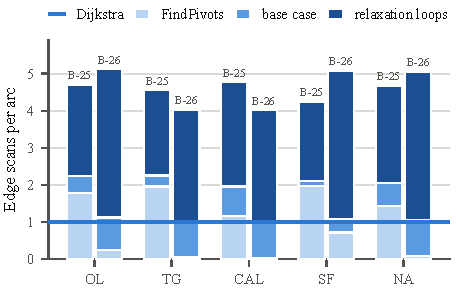
\includegraphics[width=\columnwidth]{edge_scans}
\caption{Edge scans per arc on the road networks for \bmA{} (bars marked B-25) and \bmB{}
(B-26), split by where they occur. Dijkstra's algorithm scans every arc exactly once.}
\label{fig:counts}
\end{figure}

Fig.~\ref{fig:counts} illustrates where the arc scans take place and highlights the changes
introduced by \bmB{}. In \bmA{}, \fp{} contributes more than one scan per arc across every network.
The relaxation rounds within this procedure touch each arc approximately as many times as Dijkstra's
algorithm does during its entire execution. In \bmB{}, however, the local searches account for only
a small fraction of this cost, indicating that the refinement achieves its intended purpose. These
savings are nevertheless offset by the additional work in the relaxation loops. At every level of
recursion, the algorithm relaxes all arcs leaving the sets it receives. With the prescribed
parameters, \bmB{} has one more recursion level than \bmA{} on OL, SF and NA (Table~\ref{tab:data}).
The additional topmost level simply passes the single source downward and then scans every arc once
more on the way back up.

When the time ratio is divided by the ratio of the combined number of comparisons and additions, the
resulting value represents the relative cost per counted operation. This cost ranges from
\PerOpMinTwoFive{} to \PerOpMaxTwoFive{} for \bmA{} and from \PerOpMinTwoSix{} to \PerOpMaxTwoSix{}
for \bmB{}. The overall slowdown can therefore be attributed to two factors of comparable magnitude.
First, under the comparison-addition model, \bmA{} performs \OpsRatioMinTwoFive{} to
\OpsRatioMaxTwoFive{} times more work, while \bmB{} performs \OpsRatioMinTwoSix{} to
\OpsRatioMaxTwoSix{} times more work. Second, each operation incurs additional costs that are not
captured by the model. These include the use of four-field labels instead of single numbers, the
bookkeeping required to manage blocks and tables, and less regular memory access patterns.

\subsection{Degree reduction}
Table~\ref{tab:reduce} presents the impact of applying the degree-reduction transformation to the
graph, as assumed in the theoretical analyses. With $\delta=3$, the transformed graph contains $2m$
vertices and $3m$ arcs, resulting in a vertex count that is \ReduceNGrowMin{} to \ReduceNGrowMax{}
times that of the original graph. On this transformed input, \bmA{} becomes \ReduceSlowMinTwoFive{}
to \ReduceSlowMaxTwoFive{} times slower, while \bmB{} becomes \ReduceSlowMinTwoSix{} to
\ReduceSlowMaxTwoSix{} times slower than when operating on the original graph. Dijkstra's algorithm
also experiences a slowdown of several times on the transformed input. Since the road networks
already have a maximum degree of at most 14, the transformation provides no benefit for these
networks. This observation is consistent with the findings for \bmA{} reported in~\cite{castro2025}.
Increasing the bound to $\delta=4$ reduces the performance penalty for \bmB{}, but does not
eliminate it.

\begin{table}[t]
\caption{Degree reduction: growth of the graph for $\delta=3$ and time relative to Dijkstra on
the original graph}
\label{tab:reduce}
\centering
\setlength{\tabcolsep}{3pt}
\begin{tabular}{@{}l|rr|r|rr|rrr@{}}
\hline
 & \multicolumn{2}{c|}{growth} & Dijkstra & \multicolumn{2}{c|}{\bmA} & \multicolumn{3}{c}{\bmB}\\
 & $n$ & $m$ & $\delta{=}3$ & orig. & $\delta{=}3$ & orig. & $\delta{=}3$ & $\delta{=}4$\\
\hline
\tabinput{tables/reduce.tex}
\hline
\end{tabular}
\end{table}

% Second half of the results section and the discussion (included by main.tex).

\subsection{Sensitivity to the parameters $k$ and $t$}
The parameters are prescribed for asymptotic reasons, and both papers leave their constants open. Fig.~\ref{fig:params} shows the running time on SF for all combinations of $k\in\{1,\dots,6\}$ and $t\in\{2,\dots,10\}$, with the number of levels following from $t$. Three observations hold on both SF and NA. First, $k=1$ is uniformly poor: without frontier reduction every frontier vertex goes through the recursion, and on SF the algorithms are up to \ParSFTwoFiveWorst{} (\bmA) and \ParSFTwoSixWorst{} (\bmB) times slower than Dijkstra. Second, the prescribed values are good but not the best. For \bmA{} a larger $k$ helps, which is consistent with the structure of these networks: with an average degree between 2.0 and 2.6 they consist largely of chains, and more relaxation rounds complete longer chains inside \fp. The fastest setting on SF is $k=\ParSFTwoFiveBestK$, $t=\ParSFTwoFiveBestT$ (\ParSFTwoFiveGain\% faster than prescribed) and on NA $k=\ParNATwoFiveBestK$, $t=\ParNATwoFiveBestT$ (\ParNATwoFiveGain\% faster). For \bmB{} the fastest settings use $t=\ParSFTwoSixBestT$ on both networks, which gives two levels instead of four, and are \ParSFTwoSixGain\% (SF) and \ParNATwoSixGain\% (NA) faster. Third, no setting changes the conclusion: the best ratios to Dijkstra over the whole grid are \ParSFTwoFiveBest{} and \ParSFTwoSixBest{} on SF and \ParNATwoFiveBest{} and \ParNATwoSixBest{} on NA.

\begin{figure*}[t]
\centering
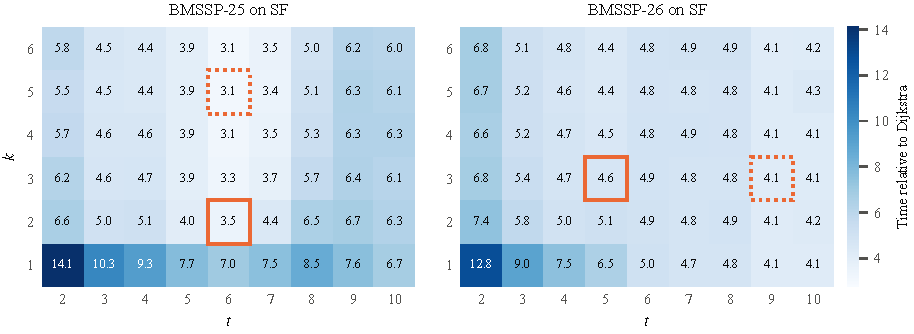
\includegraphics[width=\textwidth]{params_heatmap}
\caption{Running time relative to Dijkstra on SF for every combination of $k$ and $t$ (lighter is faster). Solid box: parameters prescribed by the respective paper; dotted box: fastest combination.}
\label{fig:params}
\end{figure*}

The topmost level of \bmB{} deserves a remark. The call one level below the top may complete up to $t^32^{(L-1)t}$ vertices, where $L=\lceil\log n/t\rceil$, and this is at least $n$ whenever $t^3\ge 2^t$, that is, for $t\le 9$. For every $n$ up to $2^{40}$ (Table~\ref{tab:params}) the top call therefore pulls the source, receives all of $V$ from its single sub-call and relaxes every arc once more without effect. This is visible in the counts: \bmB{} scans every arc once in a base case and once per level.

\subsection{Scaling on synthetic families}
Fig.~\ref{fig:scaling} shows the time relative to Dijkstra as $n$ grows from $2^{10}$ to $2^{\ScaleRandMaxExp}$ (random and grid) or $2^{\ScaleBaMaxExp}$ (preferential attachment and hub). On random digraphs the ratio falls steadily, from \ScaleRandTwoFiveFirst{} at $n=2^{10}$ to \ScaleRandTwoFiveLast{} at $n=2^{22}$ for \bmA{} and from \ScaleRandTwoSixFirst{} to \ScaleRandTwoSixLast{} for \bmB. Preferential-attachment graphs behave alike (\ScaleBaTwoFiveLast{} and \ScaleBaTwoSixLast{} at $n=2^{21}$); the heavy-tailed degree distribution makes no visible difference. On grids the improvement stops early: from $n=2^{14}$ on both algorithms stay between \GridLateMin{} and \GridLateMax{} times slower than Dijkstra. On hub graphs \bmA{} improves to \ScaleHubTwoFiveLast{} while \bmB{} is still \ScaleHubTwoSixLast{} times slower at the largest size. \bmB{} was the slower of the two new algorithms on all \SynthPoints{} synthetic instances, and neither overtakes Dijkstra anywhere in the tested range. The curves are not smooth because the prescribed $k$, $t$ and number of levels are rounded and change in steps. Above $2^{20}$ vertices the two Dijkstra variants themselves separate, the \textsc{DecreaseKey} variant becoming up to \DkLargeMax{} times slower, which indicates that at these sizes all algorithms are governed by memory-hierarchy effects that the cost model does not capture.

\begin{figure*}[t]
\centering
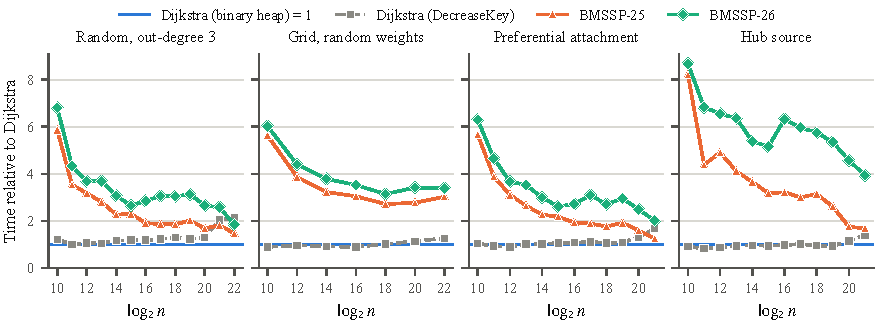
\includegraphics[width=\textwidth]{scaling_ratio}
\caption{Running time relative to Dijkstra with a binary heap on four synthetic families as a function of $n$ (geometric mean over sources).}
\label{fig:scaling}
\end{figure*}

\begin{figure*}[t]
\centering
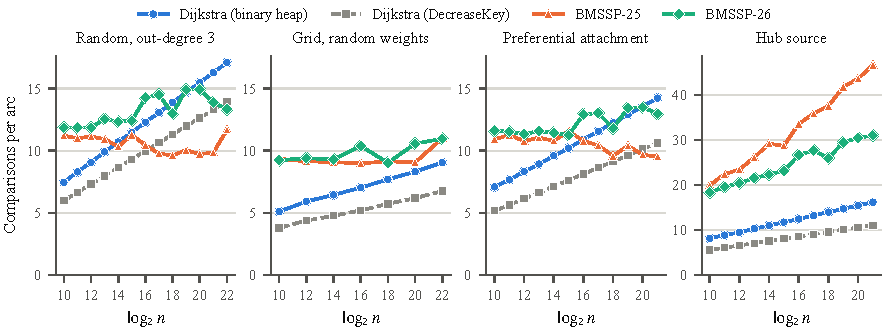
\includegraphics[width=\textwidth]{scaling_cmp}
\caption{Comparisons per arc on the synthetic families as a function of $n$. The hub family has its own vertical scale.}
\label{fig:cmp}
\end{figure*}

Fig.~\ref{fig:cmp} shows the same instances in the cost model of the theorems, and here the picture differs between families. On random and preferential-attachment graphs Dijkstra's comparisons per arc grow linearly in $\log n$, by \SlopeRandDij{} and \SlopeBaDij{} per doubling of $n$ with the lazy heap and by \SlopeRandDijDK{} and \SlopeBaDijDK{} with \textsc{DecreaseKey}. The counts of the BMSSP algorithms are nearly flat, between \CmpRangeRandTwoFiveMin{} and \CmpRangeRandTwoFiveMax{} comparisons per arc for \bmA{} and between \CmpRangeRandTwoSixMin{} and \CmpRangeRandTwoSixMax{} for \bmB{} on random graphs. The curves therefore cross: \bmA{} needs fewer comparisons than binary-heap Dijkstra at every tested size from $n=2^{\CrossCmpRandTwoFiveDij}$ on for random graphs and from $2^{\CrossCmpBaTwoFiveDij}$ on for preferential-attachment graphs ($2^{\CrossCmpRandTwoFiveDijDK}$ and $2^{\CrossCmpBaTwoFiveDijDK}$ against the \textsc{DecreaseKey} variant), and fewer comparisons plus additions from $2^{\CrossOpsRandTwoFiveDij}$ and $2^{\CrossOpsBaTwoFiveDij}$ on. \bmB{} falls below Dijkstra's comparison count at $n=2^{\CrossCmpRandTwoSixDij}$ in both families. This is the asymptotic advantage of the new algorithms appearing at feasible sizes, in the model in which it is proved. It does not carry over to running time: at $n=2^{20}$ on random graphs \bmA{} executes \OpsRandTwentyTwoFive{} comparisons and additions per arc against \OpsRandTwentyDij{} for Dijkstra and still takes \TimeRandTwentyTwoFive{} times as long. On grids and on hub graphs there is no crossing, for two different reasons discussed next.

\subsection{Graph structure: frontier width and maximum degree}\label{sec:structure}
Two properties of the input explain the differences between the families.

\emph{Frontier width.} We measure the width of Dijkstra's frontier by the largest number of vertices its indexed heap holds at any time. On the road networks this is between \RoadPeakMin\% and \RoadPeakMax\% of $n$ (Table~\ref{tab:data}), and on grids it shrinks from \PeakGridSmall\% at $n=2^{10}$ to \PeakGrid\% at $n=2^{22}$. The heap is small, extractions are cheap, and there is little ordering work for a cleverer algorithm to save; Dijkstra's algorithm makes fewer comparisons than both new algorithms at every size. On random and preferential-attachment graphs the frontier holds about \PeakRand\% and \PeakBa\% of the vertices at every size, Dijkstra's algorithm pays the logarithmic factor in full, and the counts of the new algorithms fall below it. Running time orders these inputs the same way: the smallest ratios to Dijkstra occur on random and preferential-attachment graphs, larger ones on grids and road networks.

\emph{Maximum degree.} On hub graphs the frontier is as wide as it can be, since all $n$ vertices are labelled as soon as the source is settled. Nevertheless both BMSSP algorithms need more comparisons than Dijkstra's algorithm, by a factor of \HubCmpRatioMinTwoFive{} to \HubCmpRatioMaxTwoFive{} for \bmA, increasing with $n$, and of \HubCmpRatioMinTwoSix{} to \HubCmpRatioMaxTwoSix{} for \bmB{} (Fig.~\ref{fig:cmp}, right). The counters show why. The $n-1$ arcs of the hub are relaxed together after the first base case. In \bmA{} they all fall into the range that is batch-prepended at level one, where a block holds a single key, so the structure sorts them by repeated median selection; in \bmB{} they are inserted into the search tree of the base case and handed upwards by merges. Either way the algorithm orders the entire frontier, at a higher cost per key than a heap. The analyses exclude this situation by the degree bound, which limits the number of keys one completed vertex can generate. Table~\ref{tab:hub} confirms that the bound is what is missing. After degree reduction with $\delta=3$ the instance has eight times as many vertices and satisfies the precondition, and on it \bmB{} needs fewer than half the comparisons of Dijkstra's algorithm (\HubRedCmpTwoSix{} against \HubRedCmpDij{} per arc of the original graph) and \bmA{} fewer as well (\HubRedCmpTwoFive). The advantage is real but expensive: Dijkstra's algorithm on the original graph needs only \HubCmpDij{} comparisons per arc, the transformation alone makes it \HubRedDijSlow{} times slower, and on the transformed graph \bmA{} and \bmB{} still take \HubRedSameTwoFive{} and \HubRedSameTwoSix{} times as long as Dijkstra's algorithm on the same graph.

\begin{table}[t]
\caption{Hub graph with $n=2^{18}$ as given and after degree reduction. cmp.: comparisons per arc of the original graph; time: relative to Dijkstra on the graph as given}
\label{tab:hub}
\centering
\setlength{\tabcolsep}{3.5pt}
\begin{tabular}{@{}lr|rr|rr|rr@{}}
\hline
 &  & \multicolumn{2}{c|}{Dijkstra} & \multicolumn{2}{c|}{\bmA} & \multicolumn{2}{c}{\bmB}\\
Graph & vertices & cmp. & time & cmp. & time & cmp. & time\\
\hline
\tabinput{tables/hub.tex}
\hline
\end{tabular}
\end{table}

\subsection{Web, road and social graphs}\label{sec:snap}
Table~\ref{tab:snap} repeats the comparison on \SnapGraphs{} larger real graphs. Dijkstra's algorithm is the fastest on all \SnapInstances{} instances: \bmA{} is between \SnapRatioMinTwoFive{} and \SnapRatioMaxTwoFive{} and \bmB{} between \SnapRatioMinTwoSix{} and \SnapRatioMaxTwoSix{} times slower, and \bmB{} is the faster of the two on \SnapTwoSixFaster{} of them. The closest result is \SnapBestInstance, the densest graph with the widest frontier. With unit weights, the setting in which~\cite{ryu2025} reports its simplified solver ahead of Dijkstra, the published algorithms are \SnapUnitTimeMinTwoFive{} to \SnapUnitTimeMaxTwoFive{} (\bmA) and \SnapUnitTimeMinTwoSix{} to \SnapUnitTimeMaxTwoSix{} (\bmB) times slower; we observe no advantage on any graph.

The counts follow the pattern of Section~\ref{sec:structure}. The three road networks have frontiers of at most \SnapRoadPeakMax\% of $n$, and both new algorithms need more comparisons than Dijkstra's algorithm with either weighting. The web and social graphs have frontiers between \SnapOtherPeakMin\% and \SnapOtherPeakMax\% of $n$; with random weights \bmA{} needs fewer comparisons than the lazy-heap baseline on \SnapFewerCmpTwoFive{} of them (\SnapFewerListTwoFive), the two largest. Two qualifications apply. Measured against the \textsc{DecreaseKey} variant, whose heap never holds more than $n$ entries and is therefore much cheaper on dense graphs, \bmA{} needs fewer comparisons on \SnapFewerCmpDKTwoFive{} of the \SnapInstances{} instances. And with unit weights, where Dijkstra's algorithm needs few comparisons per arc, the new algorithms need more on every graph (\SnapUnitCmpMinTwoFive{} to \SnapUnitCmpMaxTwoFive{} times for \bmA).

\begin{table}[t]
\caption{SNAP graphs. Front.: peak frontier of Dijkstra in percent of $n$ (random weights). For each of the two new algorithms: running time relative to Dijkstra with unit weights (unit) and with random weights (rand.), and comparisons relative to Dijkstra with random weights (cmp.)}
\label{tab:snap}
\centering
\setlength{\tabcolsep}{2.6pt}
\begin{tabular}{@{}lrrr|rrr|rrr@{}}
\hline
 & $n$ & $m$ & front. & \multicolumn{3}{c|}{\bmA} & \multicolumn{3}{c}{\bmB}\\
 & ($10^3$) & ($10^6$) & (\%) & unit & rand. & cmp. & unit & rand. & cmp.\\
\hline
\tabinput{tables/snap.tex}
\hline
\end{tabular}
\end{table}

\subsection{Density and weight range}
Two sweeps on random digraphs with $n=2^{18}$ vary further properties. Increasing the average out-degree from 2 to 8 lowers the ratio to Dijkstra from \DensLowTwoFive{} to \DensMinTwoFive{} for \bmA{} and from \DensLowTwoSix{} to \DensMinTwoSix{} for \bmB; beyond that the ratio stays roughly constant. Denser graphs spend a larger share of the time in plain edge scans, which all algorithms perform, but the BMSSP algorithms scan each arc three to four times, so the ratio does not approach one. The weight range has little influence: from unit weights, where all paths with the same number of arcs tie and the tie-breaking rule decides many comparisons, to weights up to $2^{30}$ the ratio stays between \WeightMinTwoFive{} and \WeightMaxTwoFive{} for \bmA{} and between \WeightMinTwoSix{} and \WeightMaxTwoSix{} for \bmB.

\subsection{Memory}
The BMSSP implementations keep one direct-address table per recursion level in addition to the labels. On the random graph with $n=2^{22}$ the peak resident set of the whole process, which includes the graph and the reference solution, is \MemDij~MB for Dijkstra, \MemTwoFive~MB for \bmA{} and \MemTwoSix~MB for \bmB, a factor of \MemRatioTwoFive{} and \MemRatioTwoSix.

\section{Discussion}\label{sec:discussion}
\emph{What \bmB{} gains over \bmA.} The redesigned \fp{} does what it promises. On the road networks it accounts for \PivotScanMinTwoSix{} to \PivotScanMaxTwoSix{} edge scans per arc, against \PivotScanMinTwoFive{} to \PivotScanMaxTwoFive{} for the relaxation rounds of \bmA. The saving is consumed by side effects of the new parameter setting. The value of $t$ is smaller than in \bmA{} (Table~\ref{tab:params}), which gives more levels, and every level relaxes all arcs once: the relaxation loops cost \MainScanMinTwoSix{} to \MainScanMaxTwoSix{} scans per arc against \MainScanMinTwoFive{} to \MainScanMaxTwoFive. In addition the base case is now a search-tree Dijkstra over up to $t^3+1$ vertices instead of a heap with a handful of entries. In total \bmB{} performs more additions than \bmA{} on \RoadsMoreAddsTwoSix{} of the five road networks and more comparisons on \RoadsMoreCmpTwoSix{} of them, and it was slower on \RealTwoSixSlowerWord{} of the five road networks and on all synthetic instances. When $t$ is chosen freely the fastest configurations of \bmB{} have two levels (Fig.~\ref{fig:params}), which suggests that the balance between $t$ and the cost of \fp{} that is optimal asymptotically is not the practical one at these sizes.

\emph{Where the time goes.} On narrow-frontier inputs the new algorithms lose twice: they execute \OpsRatioMinTwoFive{} to \OpsRatioMaxTwoFive{} (\bmA) and \OpsRatioMinTwoSix{} to \OpsRatioMaxTwoSix{} (\bmB) times as many comparisons and additions as Dijkstra's algorithm on the road networks, and each counted operation costs them \PerOpMinTwoFive{} to \PerOpMaxTwoFive{} and \PerOpMinTwoSix{} to \PerOpMaxTwoSix{} times as much time. On wide-frontier inputs of bounded degree the first handicap disappears as $n$ grows, but the second remains and by itself keeps the new algorithms behind. It is tied to features of the design that the cost model does not penalize: every arc is scanned three to five times instead of once, labels are four-field tuples instead of single numbers, and the block structures add indirection and bookkeeping. Reducing the number of passes over the arcs, for instance by skipping the redundant topmost level of \bmB, attacks the right term, but our parameter sweep indicates gains of tens of percent, not factors.

\emph{Relation to earlier measurements.} Our conclusion agrees with every study of an implementation that follows the published algorithm: \cite{castro2025} report Dijkstra to be three to four times faster on large instances, \cite{valko2025} find it faster on Lightning Network graphs, and the solver of~\cite{ryu2025} that follows the paper is reported as two to four times slower. Since our \bmA{} has the same structure as the worst-case implementation of~\cite{castro2025} (the same parameters, per-level tables and deletion repair), their published numbers also serve as a check that our implementation is not unduly slow. On random graphs with $m=3n$ they report 10.7~ms for Dijkstra and 38.2~ms for BMSSP at $n=2^{16}$, 421 and 1286~ms at $2^{20}$, and 2023 and 7703~ms at $2^{22}$ on an Intel i5-10400F; we measure \MsSixteenDij{} and \MsSixteenTwoFive~ms, \MsTwentyDij{} and \MsTwentyTwoFive~ms, and \MsTwentyTwoDij{} and \MsTwentyTwoTwoFive~ms on an Apple M1. Both of our programs are faster in absolute terms, the BMSSP implementation by the larger margin, so our ratios (\RatioRandSixteenTwoFive, \RatioRandTwentyTwoFive{} and \RatioRandTwentyTwoTwoFive) are lower than theirs (3.6, 3.1 and 3.8). The two series also differ in shape: their ratio falls from 25 at $n=2^{7}$ to about three at $2^{14}$ and then stays between 2.8 and 3.8 up to $2^{25}$, whereas ours keeps declining slowly up to $2^{22}$. The machines and graph generators differ and we did not run their code, so we cannot say whether this reflects the implementations or the hardware, and the comparison is indicative only. The reports of a practical advantage over Dijkstra that we are aware of~\cite{ryu2025,webb2025} concern simplified variants on unit-weight graphs (Section~II), and Section~\ref{sec:snap} shows no such advantage for the published algorithms on the same graphs.

\emph{Threats to validity.} All timings come from one machine and one compiler. The implementations follow the pseudocode and use sensible engineering (flat arrays, direct-address tables, no per-call allocation), but they are not tuned to the limit, and the base case of \bmB{} uses a node-based search tree because its pseudocode asks for one. The operation counts are independent of these choices only in part: they depend on the heap and selection routines used, and a heap with fewer comparisons per operation would shift Dijkstra's curves downward. Weights are integers; rounding effects of floating-point weights were not studied. The largest instances have $2^{22}$ vertices, which is far from the regime in which the asymptotic bounds separate, and we make no claim about where a crossover in running time would occur. Finally, the two observations of Section~\ref{sec:correct} concern our reading of the pseudocode of~\cite{duan2026} and have not been confirmed by its authors.


\section{Conclusion}
We compared Dijkstra's algorithm with the two algorithms proposed by Duan et al.\ that break the
sorting barrier for directed graphs. The evaluation used independent implementations, eleven real
graphs, four synthetic graph families, and operation counts under the comparison-addition model.
Across every instance, Dijkstra's algorithm with a binary heap was the fastest of the three
algorithms, with speed advantages ranging from factors of \AllRatioMin{} to \AllRatioMax. The
results under the cost model reveal a more nuanced picture. When Dijkstra's frontier is narrow, as
it is on road networks and grids, the new algorithms perform more comparisons and additions at every
tested size. However, when the frontier is wide and vertex degrees are bounded, \bmA{} performs
fewer comparisons than lazy-heap Dijkstra once the graph reaches a few tens of thousands of
vertices. This advantage appears at sizes ranging from $10^5$ to $10^6$ vertices when compared with
the \textsc{DecreaseKey} variant. \bmB{} achieves a similar advantage at approximately one million
vertices. These results show that the asymptotic advantage is real and observable on synthetic
graphs. On real web and social graphs, however, this advantage appears only against the lazy-heap
implementation and only on the two largest instances. It has not yet translated into a runtime
advantage, because every arc is scanned multiple times, and each operation incurs a higher cost.
\bmB{} achieves the lower pivot-finding cost predicted by its analysis, but with the prescribed
parameter settings, this improvement was not enough to make it faster than \bmA{} on most inputs.
The validation also revealed two cases in which the published \bmB{} pseudocode deviates from its
stated invariants. Both issues are straightforward to fix, and neither affected any computed
distance. Several useful directions for future work emerge from these findings. First,
parameter-selection rules could be developed using measured constants rather than relying solely on
asymptotic balance. Second, \bmB{} could be implemented without the redundant top level and the
node-based base case. Finally, further measurements should be conducted on machines capable of
handling graphs large enough to extend the comparison-count analysis beyond $2^{22}$ vertices.

\begin{thebibliography}{00}
\bibitem{dijkstra1959} E. W. Dijkstra, ``A note on two problems in connexion with graphs,''
\emph{Numer. Math.}, vol. 1, pp. 269--271, 1959, doi: 10.1007/BF01386390.
\bibitem{fredman1987} M. L. Fredman and R. E. Tarjan, ``Fibonacci heaps and their uses in
improved network optimization algorithms,'' \emph{J. ACM}, vol. 34, no. 3, pp. 596--615, Jul.
1987, doi: 10.1145/28869.28874.
\bibitem{driscoll1988} J. R. Driscoll, H. N. Gabow, R. Shrairman, and R. E. Tarjan, ``Relaxed
heaps: An alternative to Fibonacci heaps with applications to parallel computation,''
\emph{Commun. ACM}, vol. 31, no. 11, pp. 1343--1354, Nov. 1988, doi: 10.1145/50087.50096.
\bibitem{haeupler2024} B. Haeupler, R. Hlad\'ik, V. Rozho\v{n}, R. E. Tarjan, and J. T\v{e}tek,
``Universal optimality of Dijkstra via beyond-worst-case heaps,'' in \emph{Proc. IEEE 65th Annu.
Symp. Found. Comput. Sci. (FOCS)}, 2024, pp. 2099--2130, doi: 10.1109/FOCS61266.2024.00125.
\bibitem{duan2025} R. Duan, J. Mao, X. Mao, X. Shu, and L. Yin, ``Breaking the sorting barrier
for directed single-source shortest paths,'' in \emph{Proc. 57th Annu. ACM Symp. Theory Comput.
(STOC)}, 2025, pp. 36--44, doi: 10.1145/3717823.3718179.
\bibitem{duan2026} R. Duan, X. Mao, X. Shu, and L. Yin, ``A faster directed single-source
shortest path algorithm,'' in \emph{Proc. 53rd Int. Colloq. Automata, Lang., Program. (ICALP)},
LIPIcs, vol. 374, 2026, pp. 81:1--81:23, doi: 10.4230/LIPIcs.ICALP.2026.81.
\bibitem{castro2025} L. Castro, T. Clementino, and R. de Freitas, ``Implementation and
experimental analysis of the Duan et al. (2025) algorithm for single-source shortest paths,''
2026, arXiv:2511.03007v3.
\bibitem{valko2025} D. Valko, R. Paranjpe, and J. Marx G\'omez, ``An empirical evaluation of
BMSSP and Dijkstra's algorithm for the Lightning Network,'' 2026, arXiv:2509.13448v2.
\bibitem{makowski2025} C. Makowski, W. Guter, T. Russell, and A. Saragih, ``BMSSPy: A Python
package and empirical comparison of bounded multi-source shortest path algorithm,'' MIT Center
Transp. Logistics, Cambridge, MA, USA, Res. Paper 2025/034, Nov. 2025. [Online]. Available:
https://ssrn.com/abstract=5777186
\bibitem{cherkassky1996} B. V. Cherkassky, A. V. Goldberg, and T. Radzik, ``Shortest paths
algorithms: Theory and experimental evaluation,'' \emph{Math. Program.}, vol. 73, no. 2, pp.
129--174, May 1996, doi: 10.1007/BF02592101.
\bibitem{thorup1999} M. Thorup, ``Undirected single-source shortest paths with positive integer
weights in linear time,'' \emph{J. ACM}, vol. 46, no. 3, pp. 362--394, May 1999, doi:
10.1145/316542.316548.
\bibitem{pettie2005} S. Pettie and V. Ramachandran, ``A shortest path algorithm for
real-weighted undirected graphs,'' \emph{SIAM J. Comput.}, vol. 34, no. 6, pp. 1398--1431, 2005,
doi: 10.1137/S0097539702419650.
\bibitem{duan2023} R. Duan, J. Mao, X. Shu, and L. Yin, ``A randomized algorithm for
single-source shortest path on undirected real-weighted graphs,'' in \emph{Proc. IEEE 64th Annu.
Symp. Found. Comput. Sci. (FOCS)}, 2023, pp. 484--492, doi: 10.1109/FOCS57990.2023.00035.
\bibitem{yan2026} S. Yan, ``Lossless derandomization for undirected single-source shortest paths
and approximate distance oracles,'' in \emph{Proc. SIAM Symp. Simplicity Algorithms (SOSA)},
2026, pp. 404--412, doi: 10.1137/1.9781611978964.32.
\bibitem{kadria2026} A. Kadria and L. Roditty, ``A faster undirected single-source shortest path
algorithm,'' 2026, arXiv:2609.15247.
\bibitem{bmsspcode} L. Castro, T. Clementino, and R. de Freitas. \emph{bmssp: Header-only C++
implementation of the shortest-path BMSSP algorithm}. GitHub. Accessed: Oct. 12, 2026. [Online].
Available: https://github.com/lcs147/bmssp
\bibitem{ryu2025} M. Ryu. \emph{bmssp-python: Python implementation of the BMSSP shortest path
algorithm}. (2025). GitHub. Accessed: Oct. 12, 2026. [Online]. Available:
https://github.com/bzantium/bmssp-python
\bibitem{webb2025} J. Webb. \emph{DunMaoSSSP: A Rust implementation of the Duan--Mao et al.
algorithm for single-source shortest paths}. (2025). GitHub. Accessed: Oct. 12, 2026. [Online].
Available: https://github.com/alphastrata/DunMaoSSSP
\bibitem{frederickson1983} G. N. Frederickson, ``Data structures for on-line updating of minimum
spanning trees,'' in \emph{Proc. 15th Annu. ACM Symp. Theory Comput. (STOC)}, 1983, pp.
252--257, doi: 10.1145/800061.808754.
\bibitem{williams1964} J. W. J. Williams, ``Algorithm 232: Heapsort,'' \emph{Commun. ACM}, vol.
7, no. 6, pp. 347--348, Jun. 1964.
\bibitem{guibas1978} L. J. Guibas and R. Sedgewick, ``A dichromatic framework for balanced
trees,'' in \emph{Proc. 19th Annu. Symp. Found. Comput. Sci. (SFCS)}, 1978, pp. 8--21, doi:
10.1109/SFCS.1978.3.
\bibitem{blum1973} M. Blum, R. W. Floyd, V. Pratt, R. L. Rivest, and R. E. Tarjan, ``Time bounds
for selection,'' \emph{J. Comput. Syst. Sci.}, vol. 7, no. 4, pp. 448--461, Aug. 1973, doi:
10.1016/S0022-0000(73)80033-9.
\bibitem{musser1997} D. R. Musser, ``Introspective sorting and selection algorithms,''
\emph{Softw. Pract. Exper.}, vol. 27, no. 8, pp. 983--993, Aug. 1997.
\bibitem{thiscode} Anmol, Tanmay Arora, Adhyyan, and Pahul Veer Singh Gogna.
\emph{bmssp-vs-dijkstra: Implementations, experiments and data for a comparison of Dijkstra's
algorithm and the SSSP algorithms of Duan et al.} (2026). GitHub. Accessed: Oct. 12, 2026.
[Online]. Available: https://github.com/anmoltutejagithub/bmssp-vs-dijkstra
\bibitem{li2005} F. Li, D. Cheng, M. Hadjieleftheriou, G. Kollios, and S.-H. Teng, ``On trip
planning queries in spatial databases,'' in \emph{Advances in Spatial and Temporal Databases
(SSTD)}, Lecture Notes Comput. Sci., 2005, pp. 273--290, doi: 10.1007/11535331\_16.
\bibitem{ansari2020} M. Ansari, 2020, ``Real dataset shortest path sample (road networks of the
SSTD 2005 collection),'' GitHub. [Online]. Available:
https://github.com/mehdi-ansari/Real-dataset-shortest-path-sample
\bibitem{brinkhoff2002} T. Brinkhoff, ``A framework for generating network-based moving
objects,'' \emph{GeoInformatica}, vol. 6, no. 2, pp. 153--180, Jun. 2002, doi:
10.1023/A:1015231126594.
\bibitem{snap} J. Leskovec and A. Krevl, Jun. 2014, ``SNAP datasets: Stanford large network
dataset collection,'' Stanford Univ. [Online]. Available: http://snap.stanford.edu/data
\bibitem{barabasi1999} A.-L. Barab\'asi and R. Albert, ``Emergence of scaling in random
networks,'' \emph{Science}, vol. 286, no. 5439, pp. 509--512, Oct. 1999, doi:
10.1126/science.286.5439.509.
\bibitem{bellman1958} R. Bellman, ``On a routing problem,'' \emph{Quart. Appl. Math.}, vol. 16,
no. 1, pp. 87--90, 1958.
\end{thebibliography}

\end{document}
